\subsubsection{Encryption - Resources} \label{subsection:counter-replace-encryption-content-resource}
The first approach is to apply encryption on the application's static resources.
This can include the application's hard coded strings or image assets.
Whenever a resource is used, it has to be decrypted first.
The increase in security comes at the cost of decreased performance.
\newline
As long as application critical strings, like server addresses are encrypted, the application is unable to work.
In case no critical strings are present, the application will work as usual, but the user will not understand the application because all strings or images are still encrypted and have no meaning.
\newline
Figure~\ref{fig:encryptionResource} shows the abstract implementation of resource decryption.
\begin{figure}[h]
    \centering
    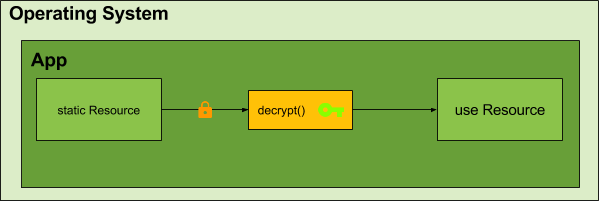
\includegraphics[width=0.8\textwidth]{data/encryptionResource.png}
    \caption{Encrypted resources have to be decrypted before they are used or displayed}
    \label{fig:encryptionResource}
\end{figure}
